%%%%%%%%%%%%%%%%%%%%%%%%%%%%%%%%%%%%%%%%%%%%%%%%%%%%%%%%%%%%%%%%%%%%%%%%%%%

\documentclass{standalone}

\usepackage{amsmath}
\usepackage{mathptmx}
\usepackage{pgfplots}
\usetikzlibrary{external}
\tikzexternalize{fermium250}
\pgfplotsset{compat=1.16}

%% IEEE uses Times Roman font, so we'll default to Times.
%% These three commands make up the entire times.sty package.
\renewcommand{\rmdefault}{ptm}
\renewcommand{\ttdefault}{pcr}
\normalfont\selectfont

\begin{document}

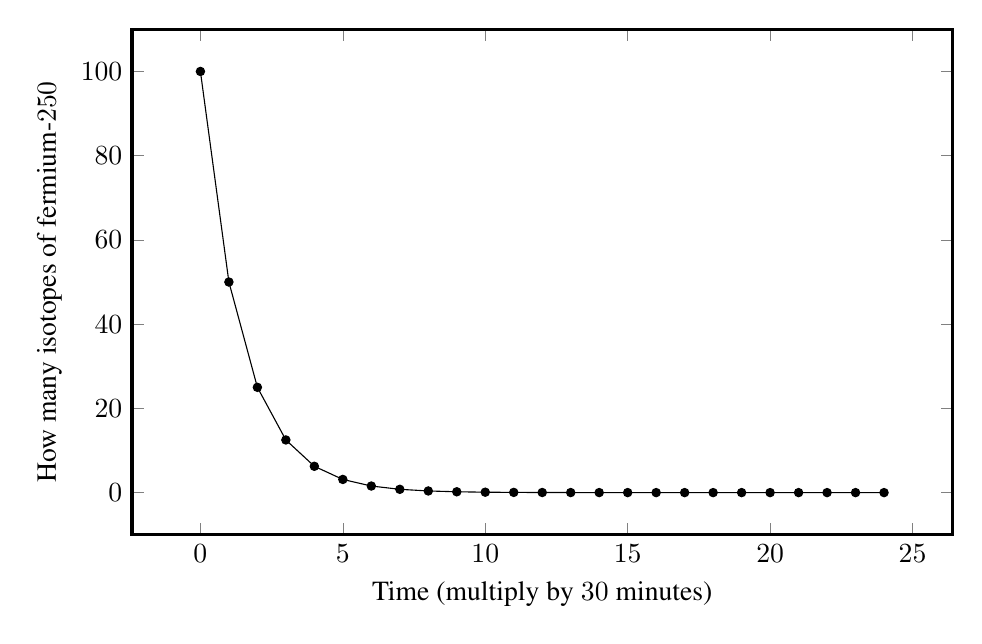
\begin{tikzpicture}
\tikzset{%%
  every mark/.append style={scale=1.0},%%
  scale=1.0%%
}
\pgfplotsset{%%
  every axis/.append style={font=\normalsize}%%
}
%%
\begin{axis}[%%
  axis line style=very thick,%%
  dotStyle/.style={mark size=1.5,black,mark color=black,mark=*},%%
  enlargelimits=true,%%
  height=8cm,%%
  width=12cm,%%
  %% x axis
  xlabel={\normalsize Time~(multiply by $30$ minutes)},%%
  %% y axis
  ylabel={\normalsize How many isotopes of fermium-$250$},%%
  scaled y ticks=false,%%
  y tick label style=/pgf/number format/fixed%%
]
%%
%%
\addplot[dotStyle] coordinates {
  (0, 100.000000)
  (1, 50.000000)
  (2, 25.000000)
  (3, 12.500000)
  (4, 6.250000)
  (5, 3.125000)
  (6, 1.562500)
  (7, 0.781250)
  (8, 0.390625)
  (9, 0.195312)
  (10, 0.097656)
  (11, 0.048828)
  (12, 0.024414)
  (13, 0.012207)
  (14, 0.006104)
  (15, 0.003052)
  (16, 0.001526)
  (17, 0.000763)
  (18, 0.000381)
  (19, 0.000191)
  (20, 0.000095)
  (21, 0.000048)
  (22, 0.000024)
  (23, 0.000012)
  (24, 0.000006)
};
\end{axis}
\end{tikzpicture}

\end{document}
